\selectlanguage{british}%

\chapter{An Alternative to Contextuality\label{chap:An-Alternative-to-Contextuality}}


\section{Rationale}

In principle, we have achieved what we set out to; we were able to
understand how BM explains PM, a test of contextuality. Having clarified
various concepts through the heavy machinery of BM, here we attempt
to further our understanding, without using BM. We will start with
refining the assumptions of the PM test. We will see how, when one
of the assumptions is refined, one version holds for QM. The other
is not even experimentally testable. Thereafter, we construct simple
toy models, one of which is unambiguously non-contextual (unlike BM,
where one must restrict the measurement process to make the same claim).
This is used to demonstrate the distinction between the two versions
of multiplicativity. We then generalize this toy model to produce
statistics consistent with QM, for an arbitrary, but discrete Hilbert
space. Finally, we generalize this to continuous variables (without
spins) and obtain a consistent one dimensional completion of QM. Its
relation with other known completions (BM \& RS) are also discussed.
This model aims to facilitate easy value assignments in case of the
phase space versions of determinism and contextuality tests. These
are hard to compute from BM and RS.


\section{Multiplicativity \label{sec:Multiplicativity}}

Let us recall two assumptions from \prettyref{sec:Peres-Mermin-Revisited},
that of non invasiveness and multiplicativity. Let $\hat{B}_{1},\hat{B}_{2},\dots,\hat{B}_{n}$
be a set of commuting observables and also let $m_{i}(\hat{*})$ represent
the value assigned to an operator. When $m$ occurs multiple times
in a given expression, then $i$ encodes the sequence of measurements.
If we assume non invasiveness, then multiplicativity has a clear meaning; 
\begin{defn*}
In a Hilbert space $\mathcal{H}$, a map $m_{i}$ from $\mathcal{H}\otimes\mathcal{H}^{\dagger}$
$\to$ $\mathbb{R}$, is \emph{multiplicative} iff 
\begin{equation}
m_{1}(f(\hat{B}_{1},\hat{B}_{2},\dots\hat{B}_{n}))=f(m_{1}(\hat{B}_{1}),m_{1}(\hat{B}_{2}),\dots m_{1}(\hat{B}_{n})).\label{eq:multiplicativity}
\end{equation}

\end{defn*}
Here we have generalized the notion from simply a product to any arbitrary
function. We have used $1$ as the subscript for each $m$, since
in this case, the sequence of a measurement is irrelevant. If one
relaxes the no-disturbance assumption, then the following also becomes
a possibility.
\begin{defn*}
In a Hilbert space $\mathcal{H}$, a map $m_{i}$ from $\mathcal{H}\otimes\mathcal{H}^{\dagger}$
$\to$ $\mathbb{R}$, is \emph{sequentially-multiplicative} iff 
\begin{equation}
m_{1}(f(\hat{B}_{1},\hat{B}_{2},\dots,\hat{B}_{n}))=f(m_{k_{1}}(\hat{B}_{1}),m_{k_{2}}(\hat{B}_{2}),\dots m_{k_{n}}(\hat{B}_{n})),\label{eq:seqMultiplicativity}
\end{equation}
where $\mathbf{k}\equiv(k_{1},k_{2},\dots k_{n})\in\{(1,2,3,\dots n),(2,1,3,\dots n),$
+ all permutations$\}$.
\end{defn*}
We take a moment to understand the meaning of these statements more
carefully, in the context of QM. Consider the state $\left|\chi\right\rangle =\left|00\right\rangle $,
$\hat{B}_{1}\equiv\hat{\sigma}_{x}\otimes\hat{\sigma}_{y}$ and $\hat{B}_{2}\equiv\hat{\sigma}_{y}\otimes\hat{\sigma}_{x}$
while $\hat{C}\equiv f(\hat{B}_{1},\hat{B}_{2})=\hat{B}_{1}\hat{B}_{2}=\hat{\sigma}_{z}\otimes\hat{\sigma}_{z}$.
Measuring $\hat{B}_{1}$ yields $\pm1$ with equal probabilities,
and so does a measurement of $\hat{B}_{2}$. However, a measurement
of $\hat{C}$ is guaranteed to yield $+1$. QM can't explicitly contradict
\prettyref{eq:multiplicativity}, since it only yields probabilities.
Further, a measurement in QM leads to disturbance, unless ofcourse
we consider simultaneous eigenstates. Therefore, after making a measurement,
say $m_{1}(\hat{B}_{1})$, one can't obtain $m_{1}(\hat{B}_{2})$.
Even if we agree to start the measurement with the same state, we
can't make the hidden variables identical. However, \prettyref{eq:seqMultiplicativity}
is certainly testable in QM, for one can first measure $\hat{B}_{1}$
to obtain $m_{1}(\hat{B}_{1})$, then measure $\hat{B}_{2}$, to find
$m_{2}(\hat{B}_{2})$ and obtain $m_{1}(\hat{B}_{1})m_{2}(\hat{B}_{2})$.
Starting from the state $\left|\chi\right\rangle $ again, one can
measure $\hat{C}$ to get $m_{1}(\hat{C})$ which has a precise value
in this case. One may again claim that experimentally, there maybe
some hidden variables which can't be made identical and thus after
measuring the $B$s, it is impossible to obtain $m_{1}(\hat{C})$.
This difficulty is circumvented in this case, by the fact that regardless
of the value of the hidden variable, given $\left|\chi\right\rangle $
and $\hat{C}$, the measurement outcome is the certain. Thus, taking
the same state $\left|\chi\right\rangle $ is enough. One can check,
from all the possibilities, if $m_{1}(\hat{B}_{1})m_{2}(\hat{B}_{2})=m_{1}(\hat{C})$.
We tried looking for states and operators that would violate this
condition, but failed. Infact, as we will prove momentarily, \emph{QM
weakly enforces sequentially multiplicative}. However, since restoring
the hidden variables is not possible in general, \emph{QM doesn't
enforce multiplicativity}.

We worked out two proofs of weak sequential multiplicativity in QM.
The first was a restricted, brute force proof. The second we showed
holds in general, which we will discuss here.
\begin{prop*}
Let the system be in a state, s.t. measurement of $\hat{C}$ yields
repeatable results (same result each time). Then according to QM,
sequential multiplicativity (see \prettyref{eq:seqMultiplicativity})
holds, where $\hat{C}\equiv f(\hat{B}_{1},\hat{B}_{2},\dots\hat{B}_{n})$,
and $\hat{B}_{i}$ are as defined. \end{prop*}
\begin{proof}
Assume without loss of generality that $\hat{B}_{1},\hat{B}_{2},\dots\hat{B}_{n}$
are mutually compatible (commuting) and complete set of operators.
If say for instance the set is not complete, then one can add the
missing operators and label them as aforesaid. It follows that $\exists$
$\left|\mathbf{b}=\left(b_{1}^{(l_{1})},b_{2}^{(l_{2})},\dots b_{n}^{(l_{n})}\right)\right\rangle $
s.t. $\hat{B}_{i}\left|\mathbf{b}\right\rangle =b_{i}^{(l_{i})}\left|\mathbf{b}\right\rangle $,
where $l_{i}$ indexes the eigenvalues corresponding to $\hat{B}_{i}$
and that $\sum_{\mathbf{b}}\left|\mathbf{b}\right\rangle \left\langle \mathbf{b}\right|=\hat{\mathbb{I}}$.
Let the state of the system be given by $\left|\psi\right\rangle $
and it must be s.t. $\hat{C}\left|\psi\right\rangle =c\left|\psi\right\rangle $,
by assumption. For the statement to follow, one need only show that
$\left|\psi\right\rangle $ must be made of only those $\left|\mathbf{b}\right\rangle $s,
which satisfy $c=f(b_{1}^{(l_{1})},b_{2}^{(l_{2})},\dots b_{n}^{(l_{n})})$.
This is the crucial step. Proving this is so is trivial. We start
with $\hat{C}\left|\psi\right\rangle =c\left|\psi\right\rangle $
and take its inner product with $\left\langle \mathbf{b}\right|$
to get 
\begin{eqnarray*}
\left\langle \mathbf{b}\right|\hat{C}\left|\psi\right\rangle  & = & c\left\langle \mathbf{b}|\psi\right\rangle ,\\
\left\langle \mathbf{b}\right|f(\hat{B}_{1},\hat{B}_{2},\dots\hat{B}_{n})\left|\psi\right\rangle  & = & c\left\langle \mathbf{b}|\psi\right\rangle ,\\
f(b_{1}^{(l_{1})},b_{2}^{(l_{2})},\dots b_{n}^{(l_{n})})\left\langle \mathbf{b}|\psi\right\rangle  & = & c\left\langle \mathbf{b}|\psi\right\rangle .
\end{eqnarray*}
Also, we have $\left|\psi\right\rangle =\sum_{\mathbf{b}}\left\langle \mathbf{b}|\psi\right\rangle \left|\mathbf{b}\right\rangle $,
from completeness. If we consider $\left|\mathbf{b}\right\rangle $s
for which $\left\langle \mathbf{b}|\psi\right\rangle \neq0$, then
we can conclude that indeed $c=f(b_{1}^{(l_{1})},b_{2}^{(l_{2})},\dots b_{n}^{(l_{n})})$.
However, when $\left\langle \mathbf{b}|\psi\right\rangle =0$, viz.
$\left|\mathbf{b}\right\rangle $s that are orthogonal to $\left|\psi\right\rangle $,
then nothing can be said. We can thus conclude that $\left|\psi\right\rangle $
is made only of those $\left|\mathbf{b}\right\rangle $s that satisfy
the required relation. That completes the proof.
\end{proof}
Note that we can't enforce sequential multiplicativity in general,
because of the hidden variable resetting objection that arises, which
was discussed with the example. However, in the PM case, where $\hat{R}_{i}$
and $\hat{C}_{j}$ are just $\pm\hat{\mathbb{I}}$, it follows that
all states are their eigenstates. Consequently, for these operators,
sequential multiplicativity must always hold. With the two notions
well defined, we now proceed with constructing two simple models,
which don't satisfy the non-invasive assumption.


\section{Simple Models}

We aim to distinguish the notion of contextuality and multiplicativity
by means of two simple models. These will not reproduce the statistics
as predicted by QM, but serve as examples and are generalized later.


\subsection{Contextual, Memory Model\label{sub:Contextual,-Memory-Model}}

The Memory Model presented here, is perhaps the simplest contextual
model. It is also non-multiplicative and invasive, viz. it doesn't
satisfy any of (1), (2) and (3), as listed in \prettyref{sec:Peres-Mermin-Revisited}.
The model is assumed to be sequentially multiplicative\footnote{infact according to QM, for row and column measurements, sequential
multiplicativity is a requirement}, and the assignments are made iteratively through the following algorithm.
We assume that the system has a matrix that can store values and has
a memory that can store the last 3 operators that were measured. Initially
assume that the matrix has all entries equal to $+1$. The algorithm
is that (i) upon measurement of an observable, yield the value as
saved in the matrix, (ii) append the observable in the 3 element memory
and (iii) update the matrix, once the context is known, to satisfy
the PM conditions on the rows and columns. 

Let us take a quick example to understand how things are working.
Assume we start with measuring $\hat{A}_{33}$. The system will yield
$m_{1}(\hat{A}_{33})=1$, in accordance with the values stored initially
(see \prettyref{eq:memoryAssignments}). The memory at this stage
would read $\{*,*,\hat{A}_{33}\}$. Since the context is not yet known,
the matrix is left unchanged. Say the next operator measured is $\hat{A}_{23}$.
Then $m_{2}(\hat{A}_{23})=1$, and the memory would be updated to
$\{*,\hat{A}_{33},\hat{A}_{23}\}$. The context is now known, and
we update the matrix to ensure that $m_{1}(\hat{C})=m_{1}(A_{33})m_{2}(A_{23})m_{3}(A_{13})=-1$.
Since the first measurements yielded $+1$, we update the matrix so
that $m_{3}(A_{13})=-1$ to finally obtain the correct PM constraint.
This has been summarized by the following equations.

\begin{equation}
m_{1}(\hat{A}_{ij})=m_{2}(\hat{A}_{ij})\doteq\left[\begin{array}{ccc}
1 & 1 & 1\\
1 & 1 & 1\\
1 & 1 & 1
\end{array}\right],\,m_{3}(\hat{A}_{ij})\doteq\left[\begin{array}{ccc}
1 & 1 & -1\\
1 & 1 & 1\\
1 & 1 & 1
\end{array}\right].\label{eq:memoryAssignments}
\end{equation}
The reader can convince her(him)self that the assignments are indeed
consistent, regardless of which row/column is measured. There are
two remarks which need to be made. First, note this model is not multiplicative,
since $m_{1}(\hat{A}_{33})m_{1}(\hat{A}_{23})m_{1}(\hat{A}_{13})=1\neq m_{1}(\hat{C})=-1$,
by construction. Second observe that the value assigned to the observables,
depends explicitly on the context, thus the model is contextual. 


\subsection{Non-Contextual, Toy Model \label{sub:Non-Contextual-Toy-Model}}

We now discuss another simple model, which is non-contextual and still
consistent with QM. It is also non-multiplicative and invasive, viz.
assumption (1) holds, but (2) and (3) don't, as listed in \prettyref{sec:Peres-Mermin-Revisited}.
Reference to the PM square will be made, and it has been reproduced,
\[
\hat{A}_{ij}\doteq\left[\begin{array}{ccc}
\hat{\mathbb{I}}\otimes\hat{\sigma}_{x} & \hat{\sigma}_{x}\otimes\hat{\mathbb{I}} & \hat{\sigma}_{x}\otimes\hat{\sigma}_{x}\\
\hat{\sigma}_{y}\otimes\hat{\mathbb{I}} & \hat{\mathbb{I}}\otimes\hat{\sigma}_{y} & \hat{\sigma}_{y}\otimes\hat{\sigma}_{y}\\
\hat{\sigma}_{y}\otimes\hat{\sigma}_{x} & \hat{\sigma}_{x}\otimes\hat{\sigma}_{y} & \hat{\sigma}_{z}\otimes\hat{\sigma}_{z}
\end{array}\right],
\]
for convenience. The assignments are made by a three step process.\\
\quad{}1. Initial State: Choose an appropriate initial state $\left|\psi\right\rangle $
(say $\left|00\right\rangle $).\\
\quad{}2. Hidden Variable (HV): Toss a coin and assign $c=+1$ for
heads, else assign $c=-1$.\\
\quad{}3. Predictions/Assignments: For an operator $\hat{p}'\in\{\hat{A}_{ij},\hat{R}_{i},\hat{C}_{j}\,(\forall\,i,j)\}$
check if $\exists$ a $\lambda$, s.t. $\hat{p}'\left|\psi\right\rangle =\lambda\left|\psi\right\rangle $.
If $\exists$ a $\lambda$, then assign $\lambda$ as the value. Else,
assign $c$.\\
So far the model has only predicted the outcomes of measurements.
If however, a measurement is made on the system, then although we
know the result from the predictions, we must update the state $\left|\psi\right\rangle $
of the system, depending on which observable is measured and arrive
at new predictions, using the aforesaid steps. The following final
step fills precisely this gap. \\
\quad{}4. Update: Say $\hat{p}$ was observed. If $\hat{p}$ is s.t.
$\hat{p}\left|\psi\right\rangle =\lambda\left|\psi\right\rangle $,
then leave the state unchanged. Else, find $\left|p_{\pm}\right\rangle $
(eigenkets of $\hat{p}$), s.t. $\hat{p}\left|p_{\pm}\right\rangle =\pm\left|p_{\pm}\right\rangle $
and update the state $\left|\psi\right\rangle \to\left|p_{c}\right\rangle $. 

Let us explicitly apply the aforesaid algorithm, to the state $\left|\psi\right\rangle =\left|00\right\rangle $.
Say we obtained tails, and thus $c=-1$. To arrive at the assignments,
note that $\left|00\right\rangle $ is an eigenket of only $\hat{R}_{i},\hat{C}_{j}$
and $\hat{A}_{33}=\hat{\sigma}_{z}\otimes\hat{\sigma}_{z}$. Thus,
in the first iteration, all these should be assigned their respective
eigenvalues. The remaining operators must be assigned $c$ (see \prettyref{eq:toyModel}).
Two remarks are in order. First, this model is \emph{non}-multiplicative,
for $m_{1}(\hat{C}_{3})=-1\neq m_{1}(\hat{A}_{13})m_{1}(\hat{A}_{23})m_{1}(\hat{A}_{33})=1$.
Second, we must impose sequential multiplicativity as a consistency
check of the model, which in particular entails that $m_{1}(\hat{C}_{3})=m_{1}(\hat{A}_{33})m_{2}(\hat{A}_{23})m_{3}(\hat{A}_{13})$.
To illustrate this, we must choose to measure $\hat{A}_{33}$. According
to step 4, since $\left|00\right\rangle $ is an eigenstate of $\hat{A}_{33}$,
the final state remains $\left|00\right\rangle $. %
\begin{comment}
{\center {\footnotesize asb}}
\end{comment}
For the next iteration, $i=2$, say we again yield $c=-1$. Since
$\left|\psi\right\rangle $ is also unchanged, the assignment remains
invariant. For the final step, we choose to measure $\hat{p}=\hat{A}_{23}(=\hat{\sigma}_{y}\otimes\hat{\sigma}_{y})$,
to proceed with sequentially measuring $\hat{C}_{3}$. To simplify
calculations, we note 
\[
\left|00\right\rangle =\frac{(\left|\tilde{+}\tilde{-}\right\rangle +\left|\tilde{-}\tilde{+}\right\rangle )/\sqrt{2}+(\left|\tilde{+}\tilde{+}\right\rangle +\left|\tilde{-}\tilde{-}\right\rangle )/\sqrt{2}}{\sqrt{2}},
\]
where $\left|\tilde{\pm}\right\rangle =\left|0\right\rangle \pm i\left|1\right\rangle $
(eigenkets of $\hat{\sigma}_{y}$). Since $\left|00\right\rangle $
is manifestly not an eigenket of $\hat{p}$, we must find $\left|p_{-}\right\rangle $,
since $c=-1$. It is immediate that $\left|p_{-}\right\rangle =\left(\left|\tilde{+}\tilde{-}\right\rangle +\left|\tilde{-}\tilde{+}\right\rangle \right)/\sqrt{2}=\left(\left|00\right\rangle +\left|11\right\rangle \right)/\sqrt{2}$,
which becomes the final state. \begin{landscape}
\begin{table}
\begin{equation}
\begin{array}{c|ccc}
\text{Iteration} & i=1 & i=2 & i=3\\
\left|\psi_{\text{init}}\right\rangle  & \left|00\right\rangle  & \left|00\right\rangle  & \frac{\left|00\right\rangle +\left|11\right\rangle }{\sqrt{2}}\\
\text{HV/Toss} & c=-1 & c=-1 & c=+1\\
\\
\text{Predictions} & m_{1}(\hat{A}_{ij})\doteq\left[\begin{array}{ccc}
-1 & -1 & -1\\
-1 & -1 & -1\\
-1 & -1 & +1
\end{array}\right] & m_{2}(\hat{A}_{ij})\doteq\left[\begin{array}{ccc}
-1 & -1 & -1\\
-1 & -1 & -1\\
-1 & -1 & +1
\end{array}\right] & m_{3}(\hat{A}_{ij})\doteq\left[\begin{array}{ccc}
+1 & +1 & +1\\
+1 & +1 & -1\\
+1 & +1 & +1
\end{array}\right]\\
\text{(Assignments)}\\
 & m_{1}(\hat{R}_{i}),m_{1}(\hat{C}_{j})=+1\,(j\neq3) & m_{2}(\hat{R}_{i}),m_{2}(\hat{C}_{j})=+1\,(j\neq3) & m_{3}(\hat{R}_{i}),m_{3}(\hat{C}_{j})=+1\,(j\neq3)\\
 & m_{1}(\hat{C}_{3})=-1 & m_{2}(\hat{C}_{3})=-1 & m_{3}(\hat{C}_{3})=-1\\
\text{Operator}\\
\text{Measured} & \hat{A}_{13}=\hat{\sigma}_{z}\otimes\hat{\sigma}_{z};m_{1}(\hat{A}_{13})=+1 & \quad\quad\hat{A}_{23}=\hat{\sigma}_{y}\otimes\hat{\sigma}_{y};m_{2}(\hat{A}_{23})=-1\quad\quad & \hat{A}_{33}=\hat{\sigma}_{x}\otimes\hat{\sigma}_{x};m_{3}(\hat{A}_{33})=+1\\
\\
\left|\psi_{\text{final}}\right\rangle  & \left|00\right\rangle  & \frac{\left|00\right\rangle +\left|11\right\rangle }{\sqrt{2}} & \frac{\left|00\right\rangle +\left|11\right\rangle }{\sqrt{2}}\\
\\
\\
\end{array}\label{eq:toyModel}
\end{equation}
\end{table}
\end{landscape}For the final iteration, $i=3$, say we yield $c=1$.
So far, we have $m_{1}(\hat{A}_{33})=1$ and $m_{2}(\hat{A}_{23})=-1$.
We must obtain $m_{3}(\hat{A}_{13})=1$, independent of the value
of $c$, to be consistent. Let's check that. According to step 3,
since $\hat{\sigma}_{x}\otimes\hat{\sigma}_{x}\left(\left|00\right\rangle +\left|11\right\rangle \right)/\sqrt{2}=1\left(\left|00\right\rangle +\left|11\right\rangle \right)/\sqrt{2}$,
$m_{3}(\hat{A}_{13})=1$ indeed. As a remark, it maybe emphasised
that the $m_{2}(\hat{A}_{33})=m_{3}(\hat{A}_{33})$ and $m_{2}(\hat{A}_{23})=m_{3}(\hat{A}_{23})$,
which essentially expresses compatibility of these observables, viz.
measurement of $\hat{A}_{13}$ doesn't affect the result one would
obtain by measuring operators compatible to it (granted they have
been measured once before). 

While this model serves as a simple counter-example to the usual `QM
is contextual' conclusion one draws the PM situation, the model fails
to yield the appropriate statistics. For instance, if we consider
simply the state $\sqrt{2}\left|\psi\right\rangle =\cos\theta\left|++\right\rangle +\sin\theta\left|--\right\rangle $,
then it follows that a measurement of $\hat{A}_{11}=\hat{\mathbb{I}}\otimes\hat{\sigma}_{x}$,
would yield $\pm1$ with equal probability according to the toy model,
whereas it (the probabilities) should depend on $\theta$ according
to QM.\footnote{This was pointed out by Prof. Arvind.}


\section{Generic Models}

In this section, we present arguably, the simplest HV theories, one
of which is for spin like systems (discrete Hilbert space) while the
other is for phase space (continuous Hilbert Space) for spin-less
particles. These models are essentially non-contextual completions
of QM, which facilitate easy computation of value assignment to operators.


\subsection{Discretely C-ingle Theory \label{sub:Discretely-C-ingle-Theory}}

The state of the system is $\left|\chi\right\rangle $, defined on
a discrete Hilbert space (spin like) and we wish to assign a value
to an arbitrary operator $\hat{A}=\sum_{a}a\left|a\right\rangle \left\langle a\right|$,
which has eigenvalues $\{a_{\text{min}}=a_{1}\le a_{2}\dots\le a_{n}=a_{\text{max}}\}$.
This theory has the following postulates: \\
1. Initial HV: Pick a $c\in[0,1]$, from a uniform random distribution.\\
2. Assignment/Prediction: The value assigned to $\hat{A}$ is given
by finding the smallest $a$ s.t. 
\[
c\le\sum_{a'=a_{\text{min}}}^{a}\left|\left\langle a'|\chi\right\rangle \right|^{2}.
\]
 A measurement of $\hat{A}$, would yield $a$.\\
3. Update: After measuring an operator, the state must be updated
(collapsed) in accordance with the rules of QM.

To see how this works, we restrict ourselves to a single spin case.
Say $\left|\chi\right\rangle =\cos\theta\left|0\right\rangle +\sin\theta\left|1\right\rangle $,
and $\hat{A}=\hat{\sigma}_{z}=\left|0\right\rangle \left\langle 0\right|-\left|1\right\rangle \left\langle 1\right|$.
Now, according to the postulates of this theory, $\hat{A}$ will be
assigned $+1$, if $c\le\cos^{2}\theta$, else $\hat{A}$ will be
assigned $-1$. It follows then, from $c$ being uniformly random
in $[0,1]$, that the statistics agree with predictions of QM. The
reader can convince him(her)self that the said scheme works in general,
specifically for the PM situation. 

We can clearly see that the assignment is non-contextual, since given
an operator and a state (+ the hidden variable), the value is uniquely
assigned. The assignment is non-multiplicative, because this scheme
when applied to the PM situation, becomes effectively the same as
the toy model (barring the statistics). We have already seen explicitly
that the toy-model non-multiplicative. The theory is ofcourse invasive,
for the state is updated after each measurement.


\subsection{Continuously C-ingle Theory | Preliminary}

The state of the system is $\left|\psi\right\rangle $, defined for
a single spin-less particle, and we wish to assign a value to an arbitrary
operator 
\[
\hat{A}=\int_{a_{\text{min}}}^{a_{\text{max}}}daa\left|a\right\rangle \left\langle a\right|.
\]
This theory has the following postulates: \\
1. Initial HV: Pick a $c\in[0,1]$, from a uniform random distribution.\\
2. Assignment/Prediction: The value assigned to $\hat{A}$ is given
by an $a$ that satisfies 
\[
c=\int_{a_{\text{min}}}^{a}\left|\psi(a')\right|^{2}da',
\]
where $\psi(a')=\left\langle a'|\psi\right\rangle $. A measurement
of $\hat{A}$, would yield $a$.\\
3. Update: After measuring an operator, the state must be updated
(collapsed) in accordance with the rules of QM.

The continuous variable version has some exclusive interesting features.
First, note that for $\hat{A}=\hat{q}$ (the position), one can predict
the trajectory of a particle. This is quite intuitive to observe graphically.
Say $c$ had a value as shown in the graph (see \prettyref{fig:Illustration-of-cingle})
\begin{figure}
\centering{}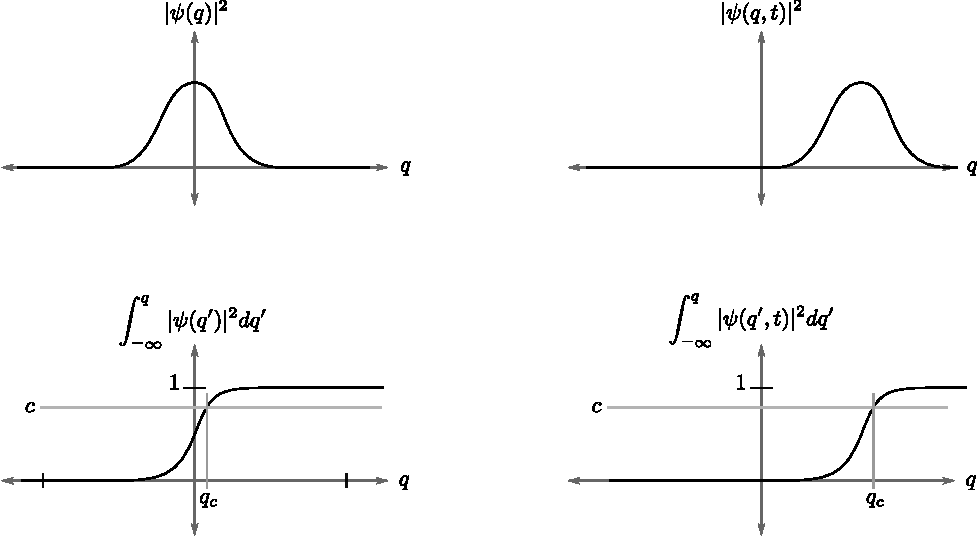
\includegraphics[width=0.95\columnwidth]{Chapter4/Figs/Vector/cingle}\caption{Illustration of the underlying principle of the continuously c-ingle
model\label{fig:Illustration-of-cingle}}
\end{figure}
and the initial state is given by a Gaussian. Now the cumulative of
this can be quickly constructed, and where the $c$ line intersects
the graph, that will yield the position of the particle. At some later
time if the Gaussian shifts (assume it had some momentum), then for
the same value of $c$, the particle's location would've moved with
the Gaussian as expected. Infact this is a general feature and can
be done for all observables, including $p$. %
\begin{comment}
Reasoning similar to the previous subsection entails that this theory
is also non-multiplicative and non-contextual.
\end{comment}
The theory is explicitly non-contextual, since values are uniquely
assigned to operators, given $\psi$ and $c$. However, one needs
more analysis to extend this to multiple particles. Once that is accomplished,
one must show that measuring the observables using the Hamiltonian
approach, would yield results consistent with those obtained from
the postulates of the theory. To show then that the theory is non-contextual,
one would be required to show that all concievable measurement schemes
would produce the same result, else, like BM, this theory wouldn't
be able to predict the values of operators with only the state and
hidden variable information. %
\begin{comment}
{[}TODO: write this section properly; the main idea is that to be
consistent with the method of measuring arbitrary observables, by
position measurements, one can't assign values in the aforesaid way.
This way, you end up with two assignments for the same observable
and have to accept eventually, that the result you get would depend
on the experiment that is performed and then there's no meaning one
can assign to an observable having a value; thus if I assign a value
to position, then effectively all my remaining freedom is lost. Thus,
one would have to restrict the theory in some, which is ok for spins,
black box the other degree of freedom, but here one can't do this.
{]}
\end{comment}
Once extended appropriately, this theory would effectively overcome
all the challenges we had for testing the continuous variable extensions
of the GHZ and contextuality tests. Predictions of observables will
be straight forward. To obtain values from BM, one had to do a detailed
analysis, for RS, evaluating values of observables other than $q$
and $p$ (even $q+p$ is hard) was hard.

We had this hunch however, that the trajectory so obtained, must be
identical to Bohmian trajectories. This infact turns out to be so.
Let us take a moment to prove this, for using the same method, one
can evalute a trajectory for the momentum also. This would be distinct
from the momentum in BM. In this case, a measurement of $\hat{p}$
yields $p$ (the assigned value), unlike in BM.
\begin{prop*}
$\dot{q}=\nabla S/m$ in a continuously c-ingle theory, for a single
particle, with one degree of freedom.\end{prop*}
\begin{proof}
Let $f$ quantify some property of a particle. To point to a particle,
we can either use the variables $c,t$ or $x,t$, since we know how
$x$ and $c$ are related. Thus, one can write $f(c,t)$ or $f(x,t)$.\footnote{If you think that the two functions should be different, then the
notation is confusing you. $f(x,t)=f(t,x)$ should help resolve. The
position of the arguments is not important, this is not like a computer
function. $f(x,t)$ is the statement that $f$ is a function of $x,t$.
That's it.} Now we have 
\[
\left[\frac{\partial f}{\partial t}\right]_{c}=\left[\frac{\partial f}{\partial t}\right]_{t}.\left[\frac{\partial q}{\partial t}\right]_{c}+\left[\frac{\partial f}{\partial t}\right]_{q},
\]
where we used $f(x,t)$ on the RHS. Note also that $\dot{q}$ refers
to the velocity of a given particle, thus it must equal $\left[\partial q/\partial t\right]{}_{c}$.
Now for $f=\int_{-\infty}^{q}\left|\psi(q')\right|^{2}dq'=c$, the
LHS disappears. Consequently, we have 
\[
\left[\frac{\partial q}{\partial t}\right]_{c}=-\left[\frac{\partial f}{\partial t}\right]_{q}/\left[\frac{\partial f}{\partial q}\right]_{t},
\]
which is in a form which can be evaluated directly from the relation
given. $\left[\partial f/\partial q\right]_{t}=\left|\psi(q,t)\right|^{2}=R^{2}$,
if $\psi=Re^{iS/\hbar}$. It is easy to show that the probability
current is given by $\nabla S/m$. Using $\left[\partial\left|\psi(q,t)\right|/\partial t\right]_{q}=-\nabla.(R^{2}\nabla S/m)$,
which is effectively the probability conservation statement, derived
from Schrodinger's equation, written in polar form, it follows that
$-\left[\partial f/\partial t\right]_{q}=R^{2}\nabla S$. Thus we
have $\dot{q}=\nabla S$ as claimed.
\end{proof}
An equation similarly for $\dot{p}$ can be obtained and an appropriate
dynamics can perhaps then be constructed. It maybe mentioned as a
remark that, quite independent of it's motivation, this scheme can
be used to compute Bohmian trajectories. It is much more efficient,
as is apparent from a comparison of the resources required between
computing an integral and the steps listed in \prettyref{sec:Bohm's-Theory,-Bohmian}.


\section{The Verdict: Contextuality vs. Non-Multiplicativity}

We have already constructed an explicit non-contextual model, which
is consistent with QM. This model we knew had to be non-multiplicative.
We will see how non-multiplicativity gives rise to what one might
confuse to mean contextuality. 

The approach is to take some compatible observables, and to construct
a `super-operator', a measurement of which can yield the values of
all of these compatible observables in a single shot. We would see
then, that the in-principle measurement outcome of observing these
compatible operators, would not be consistent. Now this one might
treat as contextuality, but according to the definition in \prettyref{sec:Peres-Mermin-Revisited},
we note that this is non-multiplicativity, as per \prettyref{sec:Multiplicativity}.

Let us construct an explicit situation and make more precise statements.
Borrowing the notation from \prettyref{sec:Multiplicativity}, imagine
\[
\hat{B}_{1}=\hat{\sigma}_{z}\otimes\hat{\mathbb{I}}=\left|00\right\rangle \left\langle 00\right|+\left|01\right\rangle \left\langle 01\right|-\left[\left|10\right\rangle \left\langle 10\right|+\left|11\right\rangle \left\langle 11\right|\right],
\]
\[
\hat{B}_{2}=\hat{\mathbb{I}}\otimes\hat{\sigma}_{z}=\left|10\right\rangle \left\langle 10\right|+\left|11\right\rangle \left\langle 11\right|-\left[\left|00\right\rangle \left\langle 00\right|+\left|01\right\rangle \left\langle 01\right|\right],
\]
while we define 
\[
\hat{C}=f(\{\hat{B}_{i}\})=0.\left|00\right\rangle \left\langle 00\right|+1.\left|01\right\rangle \left\langle 01\right|+2.\left|10\right\rangle \left\langle 10\right|+3.\left|11\right\rangle \left\langle 11\right|.
\]
$\hat{C}$ maybe viewed as a function of $\hat{B}_{1}$, $\hat{B}_{2}$
and other operators $\hat{B}_{i}$ which are constructed to obtain
a maximally commuting set. A measurement of $\hat{C}$, will collapse
the state into one of the states which are simultaneous eignkets of
$B_{1}$ and $B_{2}$. Consequently, from the observed value of $\hat{C}$,
one can deduce the values of $\hat{B}_{1}$ and $\hat{B}_{2}$. Now
consider $\sqrt{2}\left|\chi\right\rangle =\left|10\right\rangle +\left|01\right\rangle $,
for which $m_{1}(\hat{B}_{1})=1$, and $m_{1}(\hat{B}_{2})=1$, using
the discretely c-ingle theory (\prettyref{sub:Discretely-C-ingle-Theory}),
with $c<0.5$. However, $m_{1}(\hat{C})=1$, from which one can deduce
that $B_{1}$ was $+1$, while $B_{2}$ was $-1$. This property itself,
one may be tempted call contextuality, viz. the value of $B_{1}$
depends on whether it is measured alone or with the remaining $\{B_{i}\}$.
However, it must be noted that $B_{1}$ has a well defined value,
and so does $\hat{C}$. Thus by our accepted definition, there's no
contextuality. It is just that $m_{1}(\hat{C})\neq f(m_{1}(\hat{B}_{1}),m_{1}(\hat{B}_{2}),\dots)$,
viz. the theory is non-multiplicative. Note that after measuring $\hat{C}$
however, $m_{2}(\hat{B}_{1})=+1$ and $m_{2}(\hat{B}_{2})=-1$ (for
any value of $c$) consistent with those deduced by measuring $\hat{C}$.


\section{Denouement}

We have already learnt that the proof of `contextuality', infact requires
three assumptions, (1) multiplicativity, (2) non-contextuality and
(3) non-invasiveness. Here we were able to construct an explicit non-contextual
theory (for spins) which is non-multiplactive, but invasive and completely
consistent with QM. Succinctly stated, it satisfies (2) but neither
(3) nor (1), serving as a counter-example to the claim that non-contextual
hidden variable theories can't be consistent with QM. We also showed
how the theory might be misconstrued to be contextual and provided
a clarification. This is of interest because the contextuality arising
in BM from the measurement schemes, has been a source of confusion
about the said notion, arising in the PM situation.

\begin{comment}

\section{First Section of the Third Chapter}

And now I begin my third chapter here . . . And now to cite some more
people \cite{prime-number-theorem,texbook,SFPT,latex}


\subsection{First Subsection in the First Section . . .}

and some more


\subsection{Second Subsection in the First Section . . . }

and some more . . . 


\subsubsection{First subsub section in the second subsection . . . }

and some more in the first subsub section otherwise it all looks the
same doesn\textquoteright t it? well we can add some text to it .
. . 


\subsection{Third Subsection in the First Section . . . }

and some more text . . . 


\subsubsection{First subsub section in the third subsection . . . }

and some more in the first subsub section otherwise it all looks the
same doesn\textquoteright t it? well we can add some text to it and
some more and some more and some more and some more


\section{Second section with a Table}

Oh I have a table, which I can to refer (See \ref{tab:My-first-table}).

\begin{table}[H]
\hfill{}%
\begin{tabular}{|c|c|c|}
\hline 
\textbf{1} & \textbf{2} & \textbf{3}\tabularnewline
\hline 
\hline 
4 & 5 & 6\tabularnewline
\hline 
7 & 8 & 9\tabularnewline
\hline 
\end{tabular}\hfill{}

\caption{\label{tab:My-first-table}My first table (I know, it is a really
intuitive name) }
\end{table}
\end{comment}
\selectlanguage{english}%

